%
% File acl2017.tex
%
%% Based on the style files for ACL-2015, with some improvements
%%  taken from the NAACL-2016 style
%% Based on the style files for ACL-2014, which were, in turn,
%% based on ACL-2013, ACL-2012, ACL-2011, ACL-2010, ACL-IJCNLP-2009,
%% EACL-2009, IJCNLP-2008...
%% Based on the style files for EACL 2006 by
%%e.agirre@ehu.es or Sergi.Balari@uab.es
%% and that of ACL 08 by Joakim Nivre and Noah Smith

\documentclass[11pt,a4paper]{article}
\usepackage[hyperref]{acl2017}
\usepackage{times}
\usepackage{latexsym}
\usepackage{graphicx}
\usepackage{url}
\usepackage{amsmath}
\aclfinalcopy % Uncomment this line for the final submission
%\def\aclpaperid{***} %  Enter the acl Paper ID here

%\setlength\titlebox{5cm}
% You can expand the titlebox if you need extra space
% to show all the authors. Please do not make the titlebox
% smaller than 5cm (the original size); we will check this
% in the camera-ready version and ask you to change it back.

\newcommand\BibTeX{B{\sc ib}\TeX}

\title{Language Understanding System Mid Term Project}

\author{Ardino Pierfrancesco \\
  {\tt pierfrancesco.ardino@studenti.unitn.it}}

\date{}

\begin{document}
\maketitle
\begin{abstract}
    This report shows all the work done for the mid-term project for the Language Understanding System course. The project consist in developing a Spoken Language Understanding module for the Movie Domain. Different solutions have been implemented and evaluated in order to increase the performance and the accuracy on the testing set.
\end{abstract}
\section{Introduction}

The aim of this project is to develop a Spoken Language Understanding module for the Movie Domain.
The module takes as input a file composed by token-per-line sentences and produces as output the concept tag in IoB format associated to each word of a sentence. In the first part of the report the training and testing set are analyzed, extracting statistics from the two files that give some information about correlation between data. Then the solutions for compute the output are proposed. In the final section the evaluation of the solution and the comparison between them is explained.
\section{Data Analysis}
The training set and the testing set provided for this project were split into two parts:
\begin{itemize}
    \item Token-per-line set
    \item Addition Features
\end{itemize}
The first set contains sentence with word tagged with IoB concept. While the second set contains features in the following format \(Word, Lemma, PoS tag \)

\subsection{Word Distribution}
    The first kind of analysis performed on the training data is on the frequency of the words in the training set. As expected, words with a low rank have a high frequency in the training sets, also words related to the project such as the word "movie" has a high frequency in the set. Figure \ref{wordFrequency} shows the frequency of the words in the training set.

\begin{figure}[h]
    \centering
    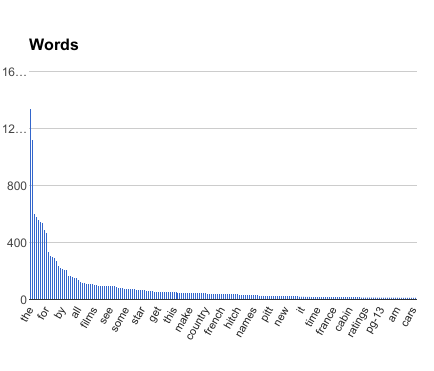
\includegraphics[width=0.6\textwidth]{image.png}
    \caption{Word frequency on training set}
    \label{wordFrequency}
\end{figure}
\subsection{Concepts distribution}
    In this section an analysis on the concept distribution is done. As can be seen from Table \ref{table} the most frequent concept is "movie.name". In this analysis the concept \texttt{"O"}, that represent the words outside of the span, is not present.
\begin{table}[h]
\centering
\begin{tabular}{l|c|r}
{\bf Concept} & {\bf Train} & {\bf Test} \\
movie.name & 3157 & 1030 \\
director.name & 455 & 156 \\
actor.name & 437 & 157 \\
producer.name & 336 & 121 \\
person.name & 280 & 66 \\
movie.subject & 247 & 59 \\
rating.name & 240 & 69 \\
country.name & 212 & 67 \\
movie.language & 207 & 72 \\
movie.release\_date & 201 & 70 \\
movie.genre & 98 & 37 \\
character.name & 97 & 21 \\
movie.gross\_revenue & 34 & 20 \\
movie.location & 21 & 11 \\
award.ceremony & 13 & 7 \\
movie.release\_region & 10 & 6  \\
actor.nationality & 6 & 1 \\
actor.type & 3 & 2 \\
director.nationality & 2 & 1 \\
movie.description & 2 & 0 \\
person.nationality & 2 & 0 \\
movie.star\_rating & 1 & 1 \\
award.category & 1 & 4 \\
movie.type & 0 & 4
\end{tabular}
\caption{Frequency of concept tags}
\label{table}
\end{table}
\section{Tools Used}
In this project to tools have been used. \texttt{OpenGRM} was used to train the language model with different combination of smoothing method and n-gram order during the simulations.
\texttt{OpenFST} was used to create the Weighted Finite State Transducers.
This project is written in \texttt{Python3} with \texttt{Bash} scripts that run each simulations.

\section{Baseline Solution}
\label{baseline}
The case of a single transducer from Word to Concept will be taken in consideration as baseline results for all the solutions. As can be seen in the Evaluation section, this is the implementation that gives acceptable performance but not so good to be taken in consideration as the final solution.

\section{Basic Project}
In this first part of the project, three transducer have been developed and tested.
\subsection{Word2Concept}
    The first transducer has been developed using only the basic training sets with only the words and the concepts. The main idea of this implementation is to use only words and concepts to computes the costs of the automaton, here words are mapped into concepts. Concepts in this case can be seen as classes that have to be predicted. \texttt{Bayesan Decision Rule} is a good candidate to achieve this goal, the Maximum Likelihood estimation has been computed has:
\begin{equation}
    P(word| IoB) = \frac{C(word, IoB)}{C(IoB)}
\end{equation}
where \textit{C(word, IoB)} is the frequency of the pair \textit{word, IoB} in the training set, while \textit{C(IoB)} is the frequency of the concept in the training set.
The Word2Concept transducer has only one state. It takes as input a word, outputs a concepts and uses as weight the minus logarithm of the likelihood computed before. The logarithm help us in the underflow problem and transform probabilities into costs. The prior probability of the concepts have been computed using the OpenGRM with different smoothing methods and n-gram size.
Unknown words have been handled giving the concepts equal proability to generate them. So the cost of a transition from an unknown word to a concept is given by:
\begin{equation}
    P(<unk> | IoB) = \frac{1}{\#IoBs}
\end{equation}
thus, 1 divided by the number of unique concepts in the training set. \\
Another solution using Frequency cut-off has been developed. Given as parameter a threshold T, all the words that appears less or equal to such a threshold have been deleted , accumulating a counter of deleted words. In this case the probability of an unknown word to be mapped into a concept is not the same for each concept, but it depends on the number of times that concept has been deleted.
\subsection{Lemma2Concept}
    This second transducer has been developed using the features training set, using the lemmas instead of the words to improve generalization. The Maximum Likelihood here is computed as:
\begin{equation}
    P(lemma| IoB) = \frac{C(lemma, IoB)}{C(IoB)}
\end{equation}
As before, the Lemma2Concept transducer has only one state that takes as input a lemma, outputs a concepts and uses as weight the minus logarithm of the likelihood computed before. Again, the prior probability has been computed using the OpenGRM tool.
\subsection{Pos2Concept}
    This final transducer has been developed using the features training set, using the Pos-tag instead of the words to see how performance changes. The Maximum Likelihood here is computed as:
\begin{equation}
    P(PoS| IoB) = \frac{C(PoS, IoB)}{C(IoB)}
\end{equation}
As before, the Pos2Concept transducer has only one state that takes as input a PoS, outputs a concepts and uses as weight the minus logarithm of the likelihood computed before. Again, the prior probability has been computed using the OpenGRM tool. As said before, the performances of this solution have been used as baseline performance.
\section{Advanced Project}
\subsection{PoSLemma2Concept}
This is the first attempt to improve the performance of the project. Here a combination of features has been used in order to improve the performance. This first test uses PoS + Lemma to train the model. Here the Maximum Likelihood is computed as:
\begin{equation}
    P(Lemma, PoS| IoB) = \frac{C(Lemma, PoS, IoB)}{C(IoB)}
\end{equation}
As before, the LemmaPos2Concept transducer has only one state that takes as input a \textit{(lemma,PoS)} pair, outputs a concepts and uses as weight the minus logarithm of the likelihood computed before. Again, the prior probability has been computed using the OpenGRM tool.
\subsection{WordLemmaPos2Concept}
This is the second attempt to improve the performance of the project. This second test uses Word + Lemma + PoS to train the model. The idea here is to use both basic and features training set to improve the accuracy of the mapping, obviously this is a risky operation as the probability of overfitting the training data is high. The Maximum Likelihood is computed as:
\begin{equation}
    \begin{split}
    P(W, L, PoS| IoB) =
                \frac{C(W, L, PoS, IoB)}{C(IoB)}
    \end{split}
    \end{equation}
As before, the WordLemmaPos2Concept transducer has only one state that takes as input a \textit{(word,lemma,PoS)} tuple, outputs a concepts and uses as weight the minus logarithm of the likelihood computed before. Again, the prior probability has been computed using the OpenGRM tool.
\subsection{Word2Concept Without O}
The last attempt to improve the performance of the project was done by removing the "O" concept from the training data and substitute the "O" assigned to a word with the word itself. By replacing the "O" concept, the model gains more information about the other tags that instead would have a low frequency compared to the "O" concept. The model is exactly the same of the Word2Concept solution, but it works on a modified training set.
\section{Evaluation and Comparison}
The evaluation of the different versions of the module has been done using as metrics accuracy,
precision, recall and F1-measure. The most important metric among the four is the F1-Score (a combination of precision and accuracy). As explained in \ref{baseline}, the Word2Concept model with unigram and \textit{unsmoothing} will be used as baseline during the evaluation. With these settings, the model has the following performance:
\begin{itemize}
    \item Accuracy: 88.84\%
    \item Precision: 55.51\%
    \item Recall:   60.04\%
    \item F1:   57.68\%
\end{itemize}
This first version analyzed is the worst among all the simulation done with the Word2concept model without cut-off.
\subsection{Word2Concept Evaluation}
Playing with the parameters of the Word2Concept model, the best performance we can reach are:
\begin{itemize}
    \item Accuracy: 92.68\%
    \item Precision: 78.51\%
    \item Recall:   74.34\%
    \item F1:   76.37\%
\end{itemize}
these performance are reached with the following parameter:
\begin{itemize}
    \item smoothing: witten\_bell
    \item ngram order: 2
\end{itemize}

While the worst performance reached with this model are the one of the baseline performance.
From all the test done using the Word2Concept model we can infer that the best smoothing method are \textit{witten\_bell} and \textit{Absolute} which give slightly better results compared to the others smoothing method. The best result are reached using bi-grams in the LM. Changing from bi-grams to unigram or tri-grams drop the performance, while using four-grams and five-grams improve the performance compared to unigram and tri-grams. Using cut-off is not a good solution, as the performance will drop considerably, so the best way to handle unknown words is using the same probabilities among all the concepts.
\subsection{Lemma2Concept Evaluation}
Playing with the parameters of the Lemma2Concept model, the best performance we can reach are:
\begin{itemize}
    \item Accuracy: 92.41\%
    \item Precision: 77.96\%
    \item Recall:   73.60\%
    \item F1:   75.72\%
\end{itemize}
these performance are reached with the following parameters:
\begin{itemize}
    \item smoothing: witten\_bell
    \item ngram order: 2
\end{itemize}

While the worst performance reached with this model are the following:
\begin{itemize}
    \item Accuracy: 87.99\%
    \item Precision: 50.13\%
    \item Recall:   53.62\%
    \item F1:   51.82\%
\end{itemize}
using the following parameters:
\begin{itemize}
    \item smoothing: unsmoothed
    \item ngram order: 1
\end{itemize}
Again, the best smoothing method are \textit{witten\_bell} and \textit{Absolute} which give slightly better results compared to the others smoothing method. The best result are reached using bi-grams in the LM. As before, changing from bi-grams to unigram or tri-grams drop the performance, while using four-grams and five-grams improve the performance compared to unigram and tri-grams.
From all the test done using the Lemma2Concept model we can infer that it has worse performance compared to the Word2Concept model. It seems that using Lemmas instead instead of words to improve generalization do not increase the performance, so we can say that this module is not a good choice for the project.
\subsection{Pos2Concept}

While using Lemmas instead of Words worse performance only by a $\sim$3\%, using PoS to train the model decrease the performance by more than the 50\%.

From the Lemma2Concept and Pos2Concept simulations we can infer that using additional features independently is not a good choice for the project as using only Words for the training phase has the best performance.

\subsection{LemmaPos2Concept}
This version of the project extended the previous one by using a combination of additional features, in this case Lemma + PoS. In this test the conclusions explained for the
basic project hold in part, in fact also in this case the \textit{witten\_bell} and \textit{absolute} resulted the best smoothing algorithms, but five-grams resulted as the best n-gram order. The best results for this module are the following:
\begin{itemize}
    \item Accuracy: 92.41\%
    \item Precision: 76.02\%
    \item Recall:   73.79\%
    \item F1:   74.88\%
\end{itemize}
using \textit{witten\_bell} as smoothing method and \textit{five-grams}
As can be seen, using a combination of Lemma and PoS do not increase the performance with respect to the Word2Concept module.

\subsection{WordLemmaPos2Concept}
As before, this version of the project use a combination of basic and additional features, in this case Word + Lemma + PoS. Also here, the conclusions of the LemmaPos2Concept test are true, in fact also in this case the \textit{witten\_bell} and \textit{absolute} resulted the best smoothing algorithms and also five-grams resulted, again, as the best n-gram order. The best results for this module are the following:
\begin{itemize}
    \item Accuracy: 92.43\%
    \item Precision: 75.99\%
    \item Recall:   73.97\%
    \item F1:   74.97\%
\end{itemize}
using \textit{witten\_bell} as smoothing method and \textit{five-grams}
As can be seen, using a combination of Words, Lemmas and PoS improves the performance of the previous test but do not reach the same performance of the Word2Concept module.

\subsection{Word2Concept without O}

This last version of the project is the one that gives the best results with respect to all the other versions. In this case the best results are reached using \textit{kneser\_ney} as smoothing method and four-grams as n gram order. The best results for this module are the following:
\begin{itemize}
    \item Accuracy: 94.96\%
    \item Precision: 82.44\%
    \item Recall:   83.04\%
    \item F1:   82.74\%
\end{itemize}
It is important to notice that all the other settings of parameters also give better results with respect to all the previous results.
This module improves the result of the baseline by 25\% in the F1-measure. As said before, removing the "O" concept from the training data gives the module the opportunity to learn more and better information about the other concept.



% include your own bib file like this:
%\bibliographystyle{acl}
%\bibliography{acl2017}

\end{document}
